\documentclass{beamer}

\usepackage{graphicx,hyperref,url}

\usepackage[T1]{fontenc}    %%% UNICODES etc
\usepackage[utf8]{inputenc}

\usepackage[portuges,brazilian]{babel}

\usepackage{booktabs}

%%%\usepackage{wrapfig}
\usepackage{caption}
\usepackage{subfigure}
\usepackage{latexsym}
\usepackage{multicol}
\usepackage{pifont}%,bbding}%%,dingbat} %%% ver manual de simbolos
\usepackage[final]{listings}
\usepackage{lmodern, comment}
\usepackage{amsmath,amssymb,amstext}
\usepackage{xcolor}

\usepackage{marvosym}

%%% FIGS
\graphicspath{ {figures/} {../ia_combinatoria/figures/} {../figures/} }
\DeclareGraphicsExtensions{.pdf,.png,.jpg}

% The log drawn in the upper right corner.

%\logo{\centering
%
\includegraphics[height=0.11\paperheight]{figures/logo02-picat.jpg}
%\hspace{0.9\paperwidth}

%%%%\graphicspath{ {/home/user} }
\definecolor{azulclaro}{rgb}{0.9,0.9,0.9}
\definecolor{mygreen}{rgb}{0,0.6,0}
\definecolor{mygray}{rgb}{0.5,0.5,0.5}
\definecolor{mymauve}{rgb}{0.58,0,0.82}
\definecolor{darkgray}{rgb}{.4,.4,.4}
\definecolor{purple}{rgb}{0.65, 0.12, 0.82}

\begin{comment}
\lstset{ 
  %  label={pgm_ex01},
    backgroundcolor=\color{azulclaro}, 
    language=Haskell, %%Miranda,%%Perl,%%%Python, %%Mercury,
    showstringspaces=false,
    basicstyle=\bf\scriptsize\ttfamily,
%%  basicstyle= \footnotesize %%% TESTAR
    keywordstyle=\textbf{\color{mygreen}}, 
    otherkeywords={*, \%, array, constraint, solve, output,  show, "/\", satisfy, set, of, if, then, elseif, float, search},
    commentstyle=\color{orange},    % comment style
     identifierstyle=\color{blue},
     stringstyle=\color{orange},
     stringstyle=\color{mymauve},
     numbers=left,  % where to put the line-numbers; possible values are (none, left, right)
      numbersep=5pt,   % how far the line-numbers are from the code
      numberstyle=\tiny\color{magenta},
      keepspaces=true      
    % %caption={LEGENDA no source PASCAL ficou OK},
}
\end{comment}

\title[Combinatorial  Optimization] % (optional, use only with long paper titlebg=blue!20!white,s)
{Programação por Restrições: \\ \textit{Um breve sobrevôo}\\ UFAL -- Maio -- 2022}
%\subtitle
%{About some things}
\author[Claudio Cesar de Sá] 
{Claudio Cesar de Sá}%\inst{1}
% - Give the names in the same order as the appear in the paper.
% - Use the \inst{?} command only if the authors have different
%   affiliation.

\institute[WhatsTV]{Independent Researcher and WhatsTV Inc.}

% - Use the \inst command only if there are several affiliations.
% - Keep it simple, no one is interested in your street address.

\date[\today] % (optional, should be abbreviation of conference name)


\begin{document}

\begin{frame}
  \titlepage
  
\end{frame}

%%%%%%%%%%%%%%%%%%%%%%%%%%
\begin{frame}[fragile]

\frametitle{Programação por Restrições}
%\label{incio_PR}

    \begin{itemize}
        \item O que é a PR?
        \item Seus princípios
        \item Onde usar? \\
       % \pause 
        R: No mundo dos NP-completos (complexidade exponencial), preferencialmente, domínios discretos $\Rightarrow$ Otimização Combinatória
        \item Contexto da IA e a PO (Pesquisa Operacional)
        \item Contexto do Brasil $\times $ cenário mundial\\ 
        onde está esta {\em turma}? onde se usa {\em isto}?
        \item As ferramentas e linguagens
        \item {\em Mãos a obra}: códigos
        \item Conclusões 
    \end{itemize}

\end{frame}

%%%%%%%%%%%%%%%%%%%%%%%%%%%%%%%%%%%%%%%%%%%%%%%%%%%%
 \begin{frame}[fragile]

\frametitle{Rápida Apresentação Minha}
\begin{itemize}
    \item Prof universitário aposentado -- UDESC
    \item Trabalhei em várias IES: entre elas a UFAL
    \item Atualmente: avô, estagiário em uma {\em start-up}, jardinagem e maratonista de águas-abertas 
    \item Interesses: CP, Picat, Linux, V, ARMs, etc
    \pause
    \item Ou seja, estou no grupo dos inquietos!
\end{itemize}

\end{frame}


%%%%%%%%%%%%%%%%%%%%%%%%%%%%%%%%%%%%%%%%%%%%%%%%%%
\begin{frame}[fragile]
%[fragile, allowframebreaks=0.9]

 \frametitle{Programação por Restrições (PR)}

   \begin{block}{}
     \begin{itemize}
     
      \item A \textcolor{magenta}{Programação por Restrições} (PR) é conhecida por \textcolor{magenta}{\textit{Constraint Programming}} 
      ou simplesmente \textbf{CP}
      
      \item {\em Restrição} em inglês é {\em restriction}, só que tem  a conotação é área, espaço, delimitação, etc, de algo que não é permitido ou seja restrito. O que não se relaciona com {\em constraint} do inglês.
      
      \item Mas {\em constraint}  não tem um boa tradução. Algo como: {\em filtragem}, {\em encolhimento} para {\bf este} contexto é quase lá.

      \pause
      \item Uma poderosa teoria (e técnica)  que  contorna a complexidade de certos problemas exponenciais
      
             
    \end{itemize}
    
    \end{block}
    
\end{frame}



\begin{frame}[fragile]
%[fragile, allowframebreaks=0.9]

% \frametitle{Programação por Restrições (PR)}

   \begin{block}{Em termos práticos (e rápido):}
     \begin{itemize}
        \item Sim, há muitos casos de uso no Brasil: {\bf ALL} (usa o CPLEX para escalonamento e horário dos trens no sul do Brasil), {\bf TOTVS} (comprou a DATASUL, módulo de planejamento de produção: SICSTUS - PROLOG), mais rescentemente, a {\bf Mercado Livre}, usam a OR-TOOLS para roteamento, logística de depósitos e empacotamento ({\em bin packing} nas vans. Tem uma equipe considerável só neste segmento!
        
        \item IBM oferece consultoria e soluções com uma equipe enorme nesta área. Há um custo clássico da IBM.
        
        \item O pacote {\em free} de roteamento/escalonamento de veículos da Google, tem feito muitas empresas investirem, nesta direção para agregar valor aos seus  produtos. 

    \end{itemize}
    
\end{block}
    
\end{frame}


%%%%%%%%%%%%%%%%%%%%%%%%%%%%%%%%%%%%%%%%%%%%%%%%%%%%%%%%%

\begin{frame}[fragile]
%[fragile, allowframebreaks=0.9]

\frametitle{Um Algoritmo da Programação por Restrições (PR)}

   \begin{block}{}
     \begin{itemize}
     
      \item \textcolor{magenta}{\textit{Aproximadamente} } o algoritmo da \textbf{\textcolor{magenta}{PR}} é dado:
          \begin{enumerate}

            \item Avaliar algebricamente  os domínios das variáveis com suas restrições

            \item Intercala iterativamente a \textcolor{magenta}{\textsf{propagação de restrições}} com  um \textcolor{magenta}{\textsf{algoritmo de busca}}

            \item A cada variável instanciada, o processo é repetido sobre as demais variáveis, reduzindo progressivamente o espaço de busca

            \item Volte ao passo inicial até que os domínios permaneçam estáticos
            e que as variáveis apresentem instâncias consistentes
              
          \end{enumerate}
       
        \pause
       \item Uma das virtudes da \textcolor{magenta}{PR}: 
       a legibilidade e clareza em construir \textcolor{magenta}{\textbf{modelos} }
       \item Exemplo: $10x = y$ tal que $D_x = \{10..20\}$ e $D_y =\{150..170\}$, logo, a solução aqui é um cartesiano: 
       \underline {$\{(15,150) , ..., (17,170) \}$ }
       
    \end{itemize}
    
    \end{block}
    
\end{frame}
%%%%%%%%%%%%%%%%%%%%%%%%%%%%%%%%%%%%%%%%%%%%%%%%%%%%%%%%%%%%%%%%%%%%%%%%%%%%%%%%%%%%%
\begin{frame}[fragile]
%[fragile, allowframebreaks=0.9]

\frametitle{Fluxo de Cálculo da PR}

\begin{figure}[!htb]
\centering
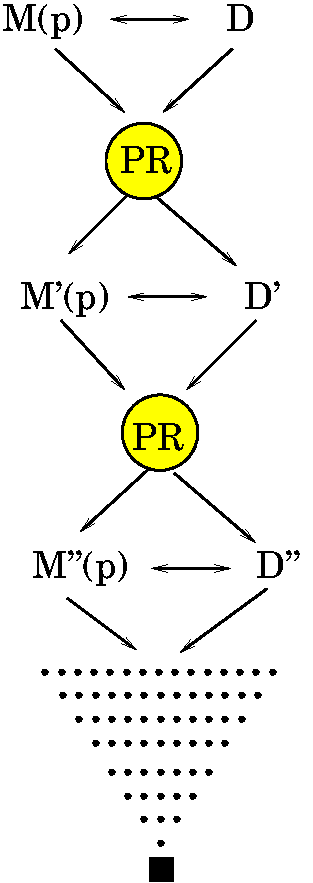
\includegraphics[width=0.30\textwidth, height=0.75\textheight]{figures/dinamica_pr.pdf}
\end{figure}
   
\end{frame}


%%%%%%%%%%%%%%%%%%%%%%%%%%%%%%%%%%%%%%%%%%%%%%%%%%%%%%%%%%%%%%%%%%%%%%%%%%%%%%%%%%%%%
\begin{frame}[fragile]
%[fragile, allowframebreaks=0.9]

\frametitle{Onde o objetivo da PR é:}

\begin{figure}[!htb]
\begin{center}
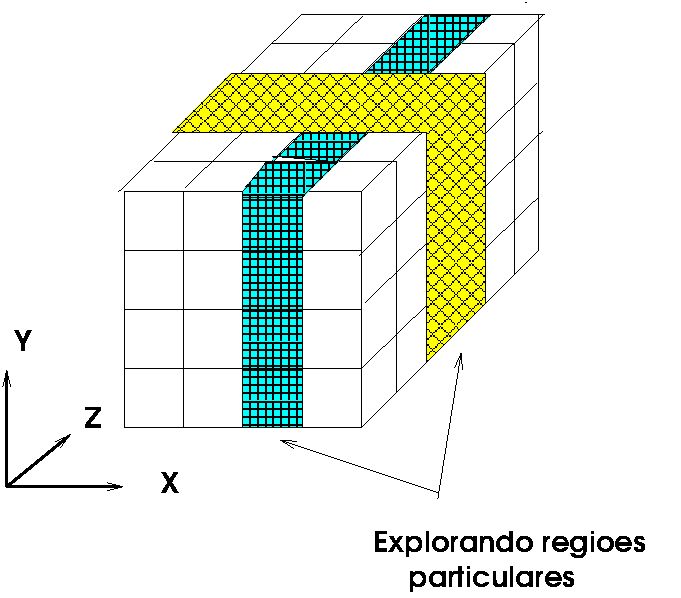
\includegraphics[width=0.70\textwidth, height=0.60\textheight]{figures/reducao_PR_01.pdf}
\caption{Realizar buscas com regiões reduzidas -- promissoras (regiões factíveis de soluções)}
\end{center}
\end{figure}
    
\end{frame}
%%%%%%%%%%%%%%%%%%%%%%%%%%%%%%%%%%%%%%%%%%%%%%%%%%%%%%%%%

\begin{frame}[fragile]
%[fragile, allowframebreaks=0.9]

\frametitle{Redução Iterativa em Sub-problemas}

\begin{figure}[!htb]

\begin{center}
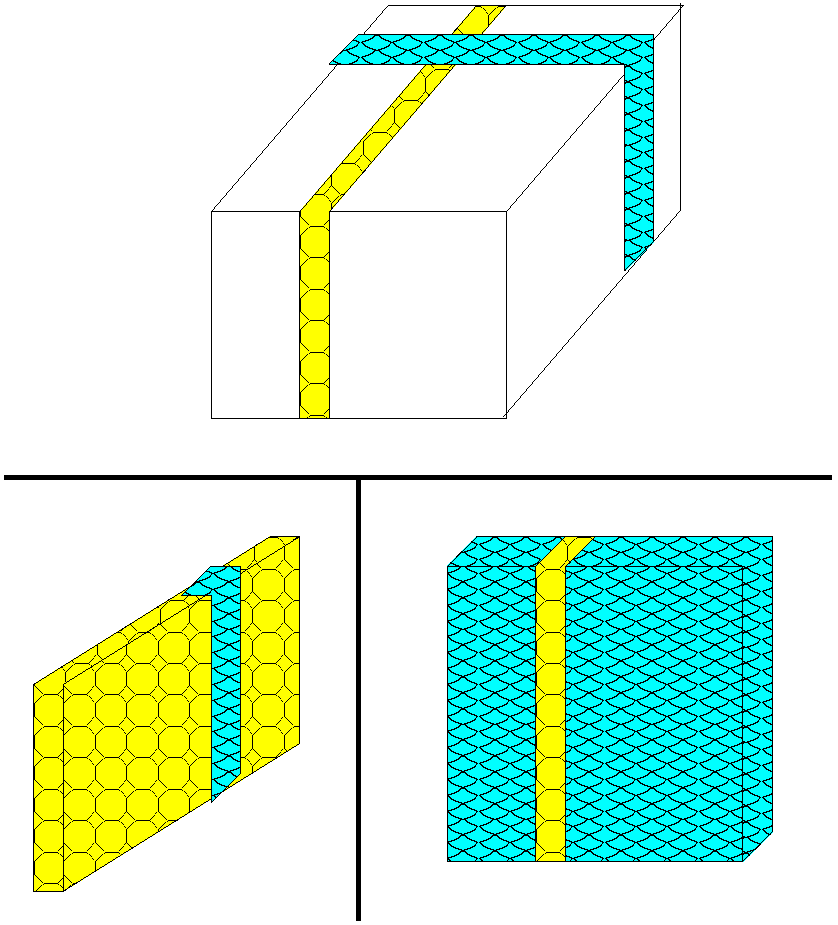
\includegraphics[width=0.70\textwidth, height=0.60\textheight]{figures/reducao_PR_02.pdf}
\caption{Redução de um CP em outros sub-problemas CPs equivalentes -- uma bisecção}
\end{center}
\end{figure}

    
\end{frame}

%%%%%%%%%%%%%%%%%%%%%%%%%%%%%%%%%%%%%%%%%%%%%%%%%%%%%%%%%%%%%%%%%%%%%%%%%%%%%%%%%%%%

\begin{frame}[fragile]
%[fragile, allowframebreaks=0.9]
\frametitle{Conceitos}

\begin{block}{A PR tem os seguintes elementos:}
    
    \begin{itemize}
    \item Um conjunto de \textbf{variáveis}: $X_1$, $X_2$, $X_3$, ..., $X_n$ 

    \item Um conjunto de \textbf{domínios} dessas variáveis: $D_{X_1}$, $D_{X_2}$, $D_{X_3}$, ..., $D_{X_n}$

    \item Finalmente, as \textbf{restrições}, que são relações n-árias entre estas variáveis

    \item Exemplo completo: $D_{X_1} = D_{X_2}= \{3,4\}$ e $X_1 \neq X_2$

\end{itemize}

\end{block}
    
\end{frame}

%%%%%%%%%%%%%%%%%%%%%%%%%%%%%%%%%%%%%%%%%%%%%%%%%%%%%%%%%%%%%%%%%%%%%%%%%%%%%%%%%%%%


\begin{frame}[fragile, allowframebreaks=0.9]

  \frametitle{Aliado a tudo isto, a CP tem um jargão todo particular:}

\begin{itemize}
    \item Problemas $\Rightarrow$ Modelos matemáticos (quase sempre, prontos para codar)
    \item Ferramentas de CP: linguagens $\times$ {\em solvers }  $\times$ bibliotecas e extensões de linguagens
    \item Sintaxe: algumas simples outras .... mas todas entendem {\bf $ 7 \#\!\!= x $} é reflexivo
    
    \item Tipagem?
    \item Domínios: inteiros? reais?
    \item Tipos de restrições: globais $\times$ a objetos
    \item Nível das restrições: simples ($a \#\!\!> b$) as complexas ($circuit (all\_vertex)$, {\texttt dfa -- exp regulares}, {\texttt soma}....
    
    \item Otimização: {\em branch-bound}
    
    \item Bisseção: ramos/trilhas por onde segue a busca
    
     \item Suporte a clones? ({\em threads})
    
    \item Reificação: condição lógica que valida uma disjunção de restrições
    
    \item {\em Channeling} : $y=f(x) \leftrightarrow x = g(y)$\\
    Exemplificando estes 2 tópicos em OR-TOOLS (Python):
  
\end{itemize}

   \begin{verbatim}
    # Criar duas restriçoes reifadas tal que : c1 <--> c2
    # c1:  b implica  (y == 10 - x).
    model.Add(y == 10 - x) . OnlyEnforceIf (b)
    # c2: not(b) implica  y == 0.
    model.Add(y == 0) . OnlyEnforceIf (b.Not())
    \end{verbatim}
   
  \begin{itemize}    
    
    \item Na CP '{\em raiz}', não há  "{\texttt if-then-else}", então a {\em reifagem} ({\em reyfing}) contorna esta dificuldade
        
    \item Finalmente:
    \begin{itemize}
        \item {\bf Escolha da sequência} da variáveis do modelo a serem exploradas
        \item {\bf Escolha} por onde se inicia a exploração dos {\bf domínios} destas variáveis
    \end{itemize}
    
  
    \item Provadores SAT, provadores lógicos baseado em LPO etc
    
    \item No meio de tudo isto, linguagens declarativas {\em cairam feito luva} $\Rightarrow$ Prolog e seus dialetos
    
    \item Resumo: CP é {\bf postar} restrições ({\bf declarar}) afim de {\em encolher} o domínio problema
    
    \item A CP quanto  há um paradigma programação (semântica):\\ $C_1 \bigwedge C_2 \bigwedge ...\bigwedge C_m \vdash \{\blacksquare_1 , ..., \blacksquare_n \} \vee \emptyset $ \\
    \noindent \textcolor{magenta}{ \rule{6cm}{10pt} }

  \end{itemize}

\end{frame}


%%%%%%%%%%%%%%%%%%%%%%%%%%%%%%%%%%%%%%%%%%%%%%%%%%%%%%%%%%%%%%%
\begin{frame}[fragile]

\frametitle{Problemas para CP na indústria}

\begin{itemize}
    \item Escalonamento e alocação de recursos
    \item Distribuição de turnos de trabalhos 
    \item Problemas de empacotamento (a van do Mercado Livre)
    \item Roteamento (veículos, cabos, paineis, placas ....)
    \item Sequenciamento de DNA (várias regras sobre sequências válidas)
    \item Planejamento financeiro
    \item Enfim: problemas que envolvam uma busca combinatória e otimização 
\end{itemize}

{\bf \textcolor{magenta}{Ou seja, ainda bem que existem os NP's !!!!}}
 
\end{frame}

%%%%%%%%%%%%%%%%%%%%%%%%%%%%%%%%%%%%
\begin{frame}[fragile]
\frametitle{A CP no Brasil}
Rapidamente:
\begin{itemize}
    \item Década de 70: primeiros doutores em CC regressam ao país
    \item Década de 80: primeiros programas de pós-graduação em CC 
    \item Década de 90: primeiros simpósios, congressos e áreas se estabelecendo
    \item Ano 2000: CAPES qualifica a pesquisa, programas, etc, indicadores de produtividade
    
    \pause
    \item {\bf \textcolor{magenta}{Aí correria começa  $\Rightarrow$ publicar !!!!}}
    \item {\bf \textcolor{magenta}{Apenas uma parte do modelo americano foi instanciado !}}
\end{itemize}

\end{frame}


\begin{frame}[fragile]
\frametitle{A CP no Brasil}

\begin{figure}[!ht]
\begin{center}
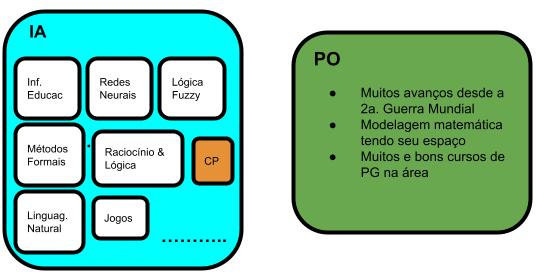
\includegraphics[width=0.90\textwidth, height=0.65\textheight]{figures/ia_brasil_90.jpg}
\caption{Cenário {\em aproximado} do borburinho em torno da {\bf IA}}
\end{center}
\end{figure}

\end{frame}

%%%%%%%%%%%%%%%%%%%%%%%%%%%%%%%%%%%%%%%%%%%%%%%%%%%%%%%%%%%%%%%
\begin{frame}[fragile]
\frametitle{A CP no Brasil}

\begin{figure}[!ht]
\begin{center}
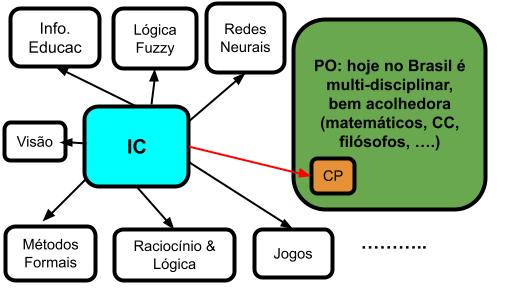
\includegraphics[width=0.90\textwidth, height=0.65\textheight]{figures/ia_brasil_2020.jpg}
\caption{A chegada dos métodos evolutivos ou bio-inspirados}
\end{center}
\end{figure}
\pause
Sim, um TSP  alcançou dimensões jamais vistas com um ACO (colônia de formigas)
\end{frame}
%
%%%%%%%%%%%%%%%%%%%%%%%%%%%%%%%%%%%%%%%%%%%%%%%%%%%%%%%%%%%%%%%


\begin{frame}[fragile, allowframebreaks=0.85]
\frametitle{Contexto Mundial}

\begin{itemize}
    \item No cenário mundial, a CP  já tinha seus nichos de sucesso na indústria. Muitas aplicações de escalonamento foram possíveis com as linguagens declarativas!
    \item Sim, o IJCAI tem a sua força de impacto!
\end{itemize}

\pause

Não em ordem de importância  e  incompleto, destacamos:
\begin{itemize}
    \item {\underline{\bf Portugal}}: {\bf LogTalk} com o Paulo Moura e o pessoal da Universidade do Porto 
    
    \item {\underline{\bf Espanha}}: Madri e Barcelona, um bom Prolog é o {\bf CIAO} (muito legal)
    
    \item {\underline{\bf França}}: pessoas espalhadas (isoladas), mas presente em quase todas universidades. Embora tenha sido o berço do Prolog, hoje os admiradores estão em Marselha apenas. Contudo, o ILOG veio de lá e foi comprado pela IBM, virou o CPLEX (muito investimento por parte da IBM), com vários cases de sucesso pelo mundo. Há outros produtos por lá: Choco (Java com CP) e Scala/JaCoP
    
    \item {\underline{\bf Alemanha}}: vários centros de pesquisa e aplicações consolidadas. Contudo, o ambiente com  {\bf Answer Set Programming}, da Universidade de Potsdam tem atraído muito a atenção. Grupo POTASCO. Usa várias lógicas para fazer inferência em seus modelos {\em ground}. Essencialmente, visa descobrir o Universo de Herbrand, por isto é conjunto de respostas!
    
    \item {\underline{\bf Itália}}: tem investido em ferramentas para o ASP. Há alguns expoentes por lá. 
    
    \item {\underline{\bf UK}}: vários centros. Destaque: Imperial College com o {\bf ECLiPSe--CLP}, contudo, Cork na Irlanda tem um grupo forte de CP. Até Oxford tem investido em ASP+Prolog+Python

    
    \item {\underline{\bf Suécia}}: uma empresa produz o SICtus Prolog, um Prolog compilado com mais de 20 anos de estrada e aplicações. Ainda ativa! {\em Gecode}: uma biblioteca em C++, muito veloz, junto com o pessoal da Alemanha mantém este resolvedor ativo, e {\bf muito bem documentado}. Na Suécia, temos ainda: Hakan Kjellerstrand -- \url{http://hakank.org}
   
    \item {\underline{\bf Noruegua}}: há uma empresa chamada PDC (Prolog compitado e tipado), com uma história de uso e sucesso. Apenas sob Windows. A PDC existe com muitos cases pela Europa.
    
    \item {\underline{\bf Holanda}}: {\bf Swi-Prolog}, do departamento de psicologia da universidade Amsterdan. Ainda ativo e mantido pelo Jan e outros. Interpretado e academicamente é o mais usado no mundo. A propósito, o Prolog é bem usado nas boas e grandes universidades pelo mundo.

   \item {\underline{\bf Polônia}}: há um livro escrito free sobre CLP -- A Gentle Guide to
Constraint Logic Programming via ECLiPSe por Antoni Niederlinski - Varsóvia
   \url{http://www.anclp.pl/download/AN_CLP.pdf}
   
   \item {\underline{\bf Tchéquia}}: em Praga há o Roman Barták (planejamento, Prolog, Picat, PDDL, etc), esteve  no NE algumas vezes

   \item {\underline{\bf USA}}: tivemos nas decadas de 80/90 Arity Prolog, Amzi Prolog, Stramberry Prolog, empresas fechadas. Restou a Google, com o OR-TOOLS (núcleo em C++) e interfaces de programação em: Java, C++, Python. Devido o investimento nos algoritmos de roteamento de veículos autônomos, hoje é a ferramenta com maior número de usuários. Seu suporte é espalhado, mas, gerenciado por Paris (resquícios do pessoal do ILOG). Há ainda o Picat de Neng-Fa e outros, como um dos principais avanços do Prolog em 40 anos. O livro do Picat está disponível ...
   
   
   \item {\underline{\bf Austrália}}: NICTA patrocina a turma CP e OR há vários anos. Ações conjuntas e um plano nacional, tornou o país de referência na área de CP. Destaque para: Peter Stuckley, Pascal Van Hentenryck, Guido, ... há um solver para OR+CP chamado FlatZinc, e sua linguagem de interface é o Minizinc.
   Hoje, os {\em aussies} (embora a maioria deles tenham vindo da Europa) ditam as várias ramificações da área de Otimização Combinatória (sim, a turma da PO está junto)
   
\end{itemize}

Em resumo: lá fora a área é ativa com várias inserções na indústria, aqui corremos atrás das publicações com qualis!

\end{frame}

%%%%%%%%%%%%%%%%%%%%%%%%%%%%%%%%%%%%%%%%%%%%%%%%%%%%%%%%%%%%%%%
\begin{frame}[fragile]
%[fragile, allowframebreaks=0.9]

\frametitle{Eventos}

\begin{itemize}
    \item CP 2022 : Principles and Practice of Constraint Programming -- Haifa -- Israel (capítulos de livros)
    
    \item CPAIOR 2022 : International Conference on the Integration of Constraint Programming, Artificial Intelligence, and Operations Research -- Los Angeles -- USA
\end{itemize}

\begin{center}
\vfill
{\bf 
\textcolor{magenta}{Até 20xx nenhum brasileiro havia publicado nestes 2 eventos!}\\
Sem qualis ...
}
\end{center}

\end{frame}

%%%%%%%%%%%%%%%%%%%%%%%%%%%%%%%%%%%%%%%%%%%%%%%%%%%%%%%%%%%%%%%%%%%%%%%%
\begin{frame}[fragile]
%[fragile, allowframebreaks=0.9]

\frametitle{Antes das {\em mãos-na-massa}:}
\begin{center}
{\large 
    Antes dos códigos, relembrando  que a CP realiza buscas, encolhendo domínios, realizando saltos a frente, ou quando voltar, sabe por onde já passou. }
    
    \vspace{1cm}
    
{\large  Ou seja, {\bf a CP é uma técnica que preza por uma busca completa}!}
    
\end{center}


\end{frame}


%%%%%%%%%%%%%%%%%%%%%%%%%%%%%%%%%%%%%%%%%%%%%%%%%%%%%%%%%%%%%%%
\begin{frame}[fragile]
%[fragile, allowframebreaks=0.9]

\frametitle{Exemplo clássico 01: Coloração de Mapas}

\begin{footnotesize}
Seja um mapa com 5 países. Cada país deve ter uma cor, mas os países
vizinhos \texttt{não} podem ter a mesma cor. 
\end{footnotesize}

\begin{figure}[!htb]
\begin{center}
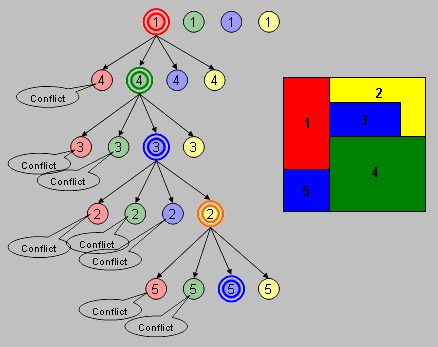
\includegraphics[width=0.750\textwidth, height=0.50\textheight]{figures/coloracao_01.jpg}
%\caption{Variáveis: . Quanto ao  Domínio? $Cores =\{1,2,3,4\}$}
\end{center}
\end{figure}

\begin{footnotesize}
\begin{itemize}
  \item \textcolor{magenta}{\textbf{Variáveis}} são os países: \texttt{X1} a \texttt{X5} -- \textbf{nós} em uma representação em grafo 
  \item Quanto ao  \textcolor{magenta}{\textbf{domínio}}? $Cores =\{1,2,3,4\}$ -- \textbf{rotulação} destes nós
  \item \textcolor{magenta}{\textbf{Restrições}}: as \textbf{arestas} de um grafo representam a relação entre países-vizinhos
\end{itemize}
\end{footnotesize}
    
\end{frame}


%%%%%%%%%%%%%%%%%%%%%%%%%%%%%%%%%%%%%%%%%%%%%%%%%%%%%%%%%%%%%%%
\begin{frame}[fragile, allowframebreaks=0.9]
%[fragile, allowframebreaks=0.9]

\frametitle{Exemplo  clássico  02: N-Rainhas no Tabuleiro $N\times N$}

\begin{figure}[!htb]
\begin{center}
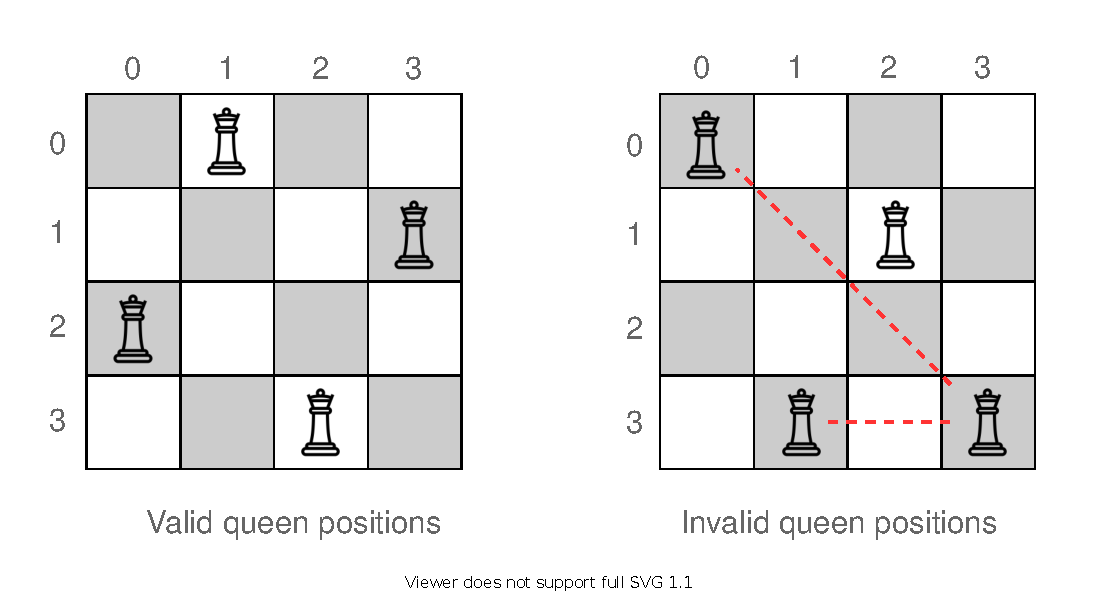
\includegraphics[width=0.580\textwidth, height=0.40\textheight]{figures/4_queens.pdf}
\caption{Distribuir 4 rainhas no tabuleiro sem se atacarem mutuamente}
\end{center}
\end{figure}



\begin{figure}[!htb]
\begin{center}
%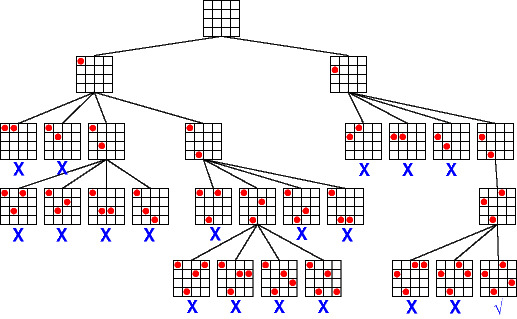
\includegraphics[width=0.70\textwidth, height=0.60\textheight]{figures/4_rainhas_01.jpg}
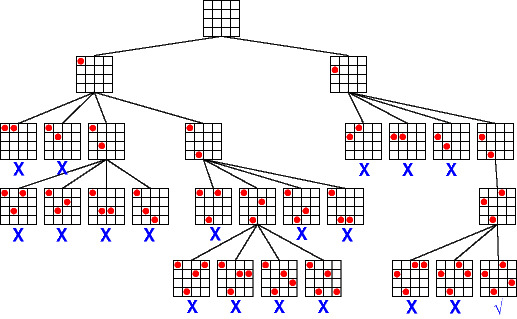
\includegraphics[width=0.490\textwidth, height=0.5\textheight]{figures/4_rainhas_01.jpg}
\hfill
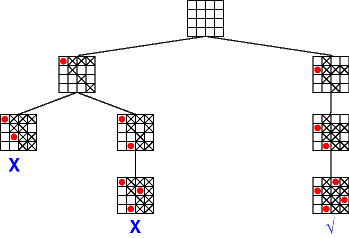
\includegraphics[width=0.490\textwidth, height=0.45\textheight]{figures/4_rainhas_02.jpg}
%\caption{Distribuir 4 rainhas no tabuleiro sem se atacarem mutuamente}
\end{center}
\end{figure}

\begin{footnotesize}
\begin{itemize}
  \item \textcolor{magenta}{\textbf{Este problema tem muitas aplicações práticas! -- uma metáfora}} 
  \item Muitas abordagens quanto ao número de variáveis e domínios
  \item Estudo sobre \textcolor{magenta}{\textbf{simetrias}} (e \textit{espelhamentos}) de na modelagem e  resultados (algo comum na PR)
\end{itemize}

\end{footnotesize}
\end{frame}



%%%%%%%%%%%%%%%%%%%%%%%%%%%%%%%%%%%%%%%%%%%%%%%%%%%%%%%%%%%%%%%
\begin{frame}[fragile] 

\frametitle{Exemplos -- {\em Mão na massa}}

Apresentando a essência dos elementos da CP na prática:

\begin{block}{}
\begin{enumerate}

  \item Um Cripto-Aritmético: um clássico escrito em Minizinc (boa para modelar) e OR-TOOLS (Python)
  
   \item Um de escala de consultórios médicos (uso de matriz)   $\Rightarrow $ em Picat (um Prolog {\em vitaminado})

\end{enumerate}
\end{block}

 \begin{center}
  \textbf{\textcolor{magenta}{Basicamente, 2 problemas distintos!}}\\

 \end{center}

\end{frame}

%%%%%%%%%%%%%%%%%%%%%%%%%%%%%%%%%%%%%%%%%%%%%%%%%%%%%%%%%%%%%%%%%%%%%%%%%%%%%%%%%%%%
\begin{frame}[fragile] 

\frametitle{Exemplo -- 01 -- Um Cripto-Aritmético}


\begin{center}
\begin{tabular}{cccccc}
V & I & O & L & I & N \\
  $-$ & C & E & L & L & O \\ \hline
C & O & R & N & E & T 
\end{tabular}
\end{center}
Preencher as letras acima, com números de $\{0..9\}$, sem repetições e que satisfaçam a a subtração  acima.
\vfill

\pause
Poderíamos transformar o problema:
\begin{center}
\begin{tabular}{cccccc}
C & O & R & N & E & T \\
 $+$ & C & E & L & L & O \\ \hline
V & I & O & L & I & N 
\end{tabular}
\end{center}

\textcolor{magenta}{Mas, vamos manter a formulação original!}

\begin{itemize}
    \item Reversabilidade (exemplo: {\texttt element(Value, L, Index))}
    \item Simetria (exemplo: n-rainhas) 
    \item Dualidade ({\em dual view}, problema da cerca -- set covering)
\end{itemize}


\end{frame}
%%%%%%%%%%%%%%%%%%%%%%%%%%%%%%%%%%%%%%%%%%%%%%%%%
\begin{frame}[fragile] 

\frametitle{Considerações sobre este clássico:}

\begin{itemize}
    \item Embora sejam {\em toy problems}, tem um viés de aplicações reais muito forte
    
    \item Efetivamente ilustram a força da CP. Como aperitivo: implemente o problema acima em uma linguagem procedural (9 laços de repetição aninhados)
    
    \item As árvores de busca ilustradas nas figuras anteriores, estão aqui presentes
    
    \item Características da CP: {\bf escolha de variável} e {\bf varredura no domínio} tem seus impactos bem visíveis nestes exemplos
    (não apresentarei estes itens)
    
\end{itemize}

\end{frame}
%%%%%%%%%%%%%%%%%%%%%%%%%%%%%%%%%%%%%%%%%%%%%%%%%
\begin{frame}[fragile] 

\frametitle{Implementação em Minizinc}

Acompanhar: \\
{\bf \textcolor{magenta}{ \url{https://raw.githubusercontent.com/claudiosa/CCS/master/minizinc/violin_cripto.mzn}}}
{\small
\begin{verbatim}
Compiling violin_cripto.mzn
Running violin_cripto.mzn
V: 7	I: 0	O: 4	L: 8	I: 0	N: 9
    C: 6	E: 2	L: 8	L: 8	O: 4
--------------------------------------------------
C: 6	O: 4	R: 1	N: 9	E: 2	T: 5

 f MAXIMIMIZACAO: 21
C1: 0	C2: 1	C3: 1	C4: 0	C5: 1
----------
==========
\end{verbatim}
}
\end{frame}
%%%%%%%%%%%%%%%%%%%%%%%%%%%%%%%%%%%%%%%%%%%%%%%%%%%%%%%%%%%%%%%%%%%%

%%%%%%%%%%%%%%%%%%%%%%%%%%%%%%%%%%%%%%%%%%%%%%%%%
\begin{frame}[fragile] 

\frametitle{Implementação em OR-TOOLS (Python)}

Acompanhar: \\
{\bf \textcolor{magenta}{ \url{https://github.com/claudiosa/CCS/blob/master/python/or-tools/violin_cripto.py}}}
{\small
\begin{verbatim}
$ python3 violin_cripto.py 
=============== RESULTS ====================
MAX = 21
V:7 || I:0 || O:4 || L:8 || N:9 || C:6 ||  E:2 ||  R:1 || T:5
carry[0] : 0 
carry[1] : 1 
carry[2] : 1 
carry[3] : 0 
carry[4] : 1 
** Final Statistics **
  - conflicts : 16
  - branches  : 29
  - wall time : 0.023359 s
\end{verbatim}
}
\end{frame}
%%%%%%%%%%%%%%%%%%%%%%%%%%%%%%%%%%%%%%%%%%%%%%%%%
\begin{frame}[fragile] 

\frametitle{Exemplo -- 02 -- Escala de Consultórios}



\begin{table}[]
\begin{tabular}{|c|c|c|c|c|c|}
\hline
{\color[HTML]{00009B} }                                 & {\color[HTML]{CB0000} \textbf{2a.}}                             & {\color[HTML]{CB0000} \textbf{3a.}}        & {\color[HTML]{CB0000} \textbf{4a.}}        & \multicolumn{1}{l|}{{\color[HTML]{CB0000} \textbf{5a.}}}        & \multicolumn{1}{l|}{{\color[HTML]{CB0000} \textbf{6a.}}}        \\ \hline
{\color[HTML]{303498} \textbf{1a. Sala}}                       & {\color[HTML]{009901} \textbf{{[}1..7{]}}}                      & {\color[HTML]{009901} \textbf{{[}1..7{]}}} & {\color[HTML]{009901} \textbf{{[}1..7{]}}} & \multicolumn{1}{l|}{{\color[HTML]{009901} \textbf{{[}1..7{]}}}} & \multicolumn{1}{l|}{{\color[HTML]{009901} \textbf{{[}1..7{]}}}} \\ \hline
{\color[HTML]{303498} \textbf{2a. Sala}}                       & {\color[HTML]{009901} \textbf{{[}1..7{]}}}                      & ...                                        & ...                                        & ...                                                             & ...                                                             \\ \hline
{\color[HTML]{303498} \textbf{3a. Sala}}                       & {\color[HTML]{009901} \textbf{{[}1..7{]}}}                      & ...                                        & ...                                        & ...                                                             & ...                                                             \\ \hline
\multicolumn{1}{|l|}{{\color[HTML]{303498} \textbf{4a. Sala}}} & \multicolumn{1}{l|}{{\color[HTML]{009901} \textbf{{[}1..7{]}}}} & ...                                        & ...                                        & ...                                                             & ...                                                             \\ \hline
\end{tabular}
\end{table}
\begin{itemize}
    
\item {\bf \textcolor{magenta}{Basicamente, alocar 7 especialidades médicas nestas 4 salas, nestes 5 dias da semana -- {\em assignment problem}}}

\item {\bf 1:oftalmo, 2:otorrino, 3:pediatra,  4:gineco, 5:cardio, 6:dermato, 7:clin\_geral}

\end{itemize}

\end{frame}

%%%%%%%%%%%%%%%%%%%%%%%%%%%%%%%%%%%%%%%%%%%%%%%%%%%%%%%%%%%%%%%

\begin{frame}[fragile] 

\frametitle{Exemplo -- 02 -- Escala de Consultórios}



\begin{itemize}
\item Seja um Posto Atendimento Médico, um PA, com 4 consultórios e 7 especialidades  médicas


\item O problema é distribuir estes médicos nestes 4 consultórios
tal que alguns requisitos sejam atendidos (restrições  satisfeitas)

\item A abordagem aqui é ingênua e sem muitos critérios (problema de minha autoria)
\end{itemize}

\end{frame}

%%%%%%%%%%%%%%%%%%%%%%%%%%%%%%%%%%%%%%%%%%%%%%%%%%
\begin{frame}[fragile] 

\frametitle{Modelagem do Problema}

\begin{itemize}
  \item  Vamos usar uma matriz bi-dimensional para 
  representar o problema. Linhas $\leftrightarrow$ consultórios (1 a 4), e 
  as colunas $\leftrightarrow$ dias da semana (1 a 5)

  
  \item Esta matriz será preenchida com valores/códigos de 1 a 7, de acordo com a especialidade médica.
  
  
  \item Assim o domínio da matriz \texttt{Quadro} ($4 \times 5$) será   preenchida com um destes códigos.
   
  
  \item Vamos utilizar restrições globais: \textcolor{magenta}{\texttt{member}} e 
  \textcolor{magenta}{\texttt{all\_different}}

   \item As restrições globais se aplicam sobre um conjunto de variáveis.

\end{itemize}

\end{frame}

%%%%%%%%%%%%%%%%%%%%%%%%%%%%%%%%%%%%%%%%%%%%%%%%%%%%%%%%%%%%%%%

\begin{frame}
  \frametitle{Matriz de Atribuição}

% Please add the following required packages to your document preamble:
% \usepackage[table,xcdraw]{xcolor}
% If you use beamer only pass "xcolor=table" option, i.e. \documentclass[xcolor=table]{beamer}
\begin{table}[]
\begin{tabular}{|c|c|c|c|c|c|}
\hline
{\color[HTML]{00009B} }                                 & {\color[HTML]{CB0000} \textbf{2a.}}                             & {\color[HTML]{CB0000} \textbf{3a.}}        & {\color[HTML]{CB0000} \textbf{4a.}}        & \multicolumn{1}{l|}{{\color[HTML]{CB0000} \textbf{5a.}}}        & \multicolumn{1}{l|}{{\color[HTML]{CB0000} \textbf{6a.}}}        \\ \hline
{\color[HTML]{303498} \textbf{1a. Sala}}                       & {\color[HTML]{009901} \textbf{{[}1..7{]}}}                      & {\color[HTML]{009901} \textbf{{[}1..7{]}}} & {\color[HTML]{009901} \textbf{{[}1..7{]}}} & \multicolumn{1}{l|}{{\color[HTML]{009901} \textbf{{[}1..7{]}}}} & \multicolumn{1}{l|}{{\color[HTML]{009901} \textbf{{[}1..7{]}}}} \\ \hline
{\color[HTML]{303498} \textbf{2a. Sala}}                       & {\color[HTML]{009901} \textbf{{[}1..7{]}}}                      & ...                                        & ...                                        & ...                                                             & ...                                                             \\ \hline
{\color[HTML]{303498} \textbf{3a. Sala}}                       & {\color[HTML]{009901} \textbf{{[}1..7{]}}}                      & ...                                        & ...                                        & ...                                                             & ...                                                             \\ \hline
\multicolumn{1}{|l|}{{\color[HTML]{303498} \textbf{4a. Sala}}} & \multicolumn{1}{l|}{{\color[HTML]{009901} \textbf{{[}1..7{]}}}} & ...                                        & ...                                        & ...                                                             & ...                                                             \\ \hline
\end{tabular}
\end{table}

O domínio de valores: \texttt{1..7} (7 especialidades médicas)

\end{frame}



%%%%%%%%%%%%%%%%%%%%%%%%%%%%%%%%%%%%%%%%%%%%%%%%%%%%%%%%%%%%%%%
\begin{frame}[fragile] 

\frametitle{Modelagem -- Comentários}

\begin{itemize}
  \item A fase de busca e propagação do comando 	\texttt{solve(Critérios, Variáveis)}, 
  há dezenas de combinações possíveis: consultar o guia do usuário
  
  
  \item Tem-se os predicados extras ... são muitos, todos os da CP

  
\end{itemize}

\end{frame}


%%%%%%%%%%%%%%%%%%%%%%%%%%%%%%%%%%%%%%%%%%%%%%%%%%%%%%%%%%%%%%%
\begin{frame}[fragile]
 \frametitle{Código Completo}

\begin{itemize}
  \item Acompanhar as explicações do código de:\\
\url{https://github.com/claudiosa/CCS/blob/master/picat/horario_medico_CP.pi}

  \item Confira a execução e testes
\end{itemize}
\end{frame}


%%%%%%%%%%%%%%%%%%%%%%%%%%%%%%%%%%%%%%%%%%%%%%%%%%%%
\begin{frame}[fragile] 

\frametitle{Código em Partes}

\begin{footnotesize}
\begin{verbatim}
modelo => 
    Dias = 5, % segunda= 1, ...., sexta-feira = 5
    Consultorio = 4,
    L_dom = [ oftalmo, otorrino, pediatra,  gineco, 
%                1        2          3         4
              cardio, dermato, clin_geral ],
%                5       6        7
   Quadro = new_array(Consultorio, Dias ), %% Lin x Col
   Quadro :: 1 .. L_dom.len , %% operador len . "eh colado"
...
\end{verbatim}

\end{footnotesize}

{\bf \textcolor{magenta}{As variáveis do problema são em letras MAIÚSCULAS, idem a Prolog}}   
    
\end{frame}
%%%%%%%%%%%%%%%%%%%%%%%%%%%%%%%%%%%%%%%%%%%%%%%%%%%%
\begin{frame}[fragile] 

\frametitle{Código em Partes}

\begin{footnotesize}
\begin{verbatim}
    %% O medico 2 NUNCA trabalha no consultorio 1
    foreach ( J in 1 .. Dias ) 
        Quadro[1,J] #!= 2
    end,
    
    %% O medico 5 NUNCA trabalha no consultorio 4
    foreach ( J in 1 .. Dias ) 
        Quadro[4,J] #!= 5
    end,

% O medico 6 soh vem na 2a (1) e 6a. (5) feira
    count( 6, [Quadro[I,1] : I in 1 .. Consultorio],1),
    count( 6, [Quadro[I,5] : I in 1 .. Consultorio],1),
\end{verbatim}
\end{footnotesize}
    
\end{frame}

%%%%%%%%%%%%%%%%%%%%%%%%%%%%%%%%%%%%%%%%%%%%%%%%%%%%%%%%%%%%%%%
\begin{frame}[fragile] 

\frametitle{Código em Partes}

\begin{footnotesize}
\begin{verbatim}

 %% O Clin Geral trabalha 2a, 4as e 6as.
 foreach ( J in {1,3,5} )
    count(7,[Quadro[I,J] : I in 1 .. Consultorio],1) 
 end, 
  
  %% Ninguém trabalha no mesmo consultorio em dias seguidos
  foreach ( J in 1 .. Dias )
      all_different( [Quadro[I,J] : I in 1..Consultorio] )
  end,  
 
  %% Ninguém trabalha no mesmo dia em mais de um consultorio
   foreach ( I in 1 .. Consultorio )
      all_different( [Quadro[I,J] : J in 1..Dias] )
   end,  
...  
\end{verbatim}
\end{footnotesize}
    
\end{frame}
%%%%%%%%%%%%%%%%%%%%%%%%%%%%%%%%%%%%%%%%%%%%%%%%%%%%
\begin{frame}[fragile] 

\frametitle{Código em Partes}

\begin{footnotesize}
\begin{verbatim}
	% A BUSCA
	solve([ff], Quadro),
  % UMA SAIDA
	
   printf("\n Uma escolha:"),
   print_matrix( Quadro ),
   print_matrix_NAMES( Quadro , L_dom ),
	 printf(".............................\n") .
\end{verbatim}
\end{footnotesize}
    
\end{frame}
%%%%%%%%%%%%%%%%%%%%%%%%%%%%%%%%%%%%%%%%%%%%%%%%%%%%
\begin{frame}[fragile] 

\frametitle{Código em Partes}

\begin{footnotesize}
\begin{verbatim}
print_matrix_NAMES( M, Lista ) =>
 L = M.length,
 C = M[1].length,
  nl,
   foreach(I in 1  .. L)
     foreach(J in 1  ..  C)
      printf(":%w \t" , print_n_lista( M[I,J], Lista) )
     % printf("(%d,%d): %w " , I, J, M[I,J] ) -- FINE
     end,
     nl
   end.
%%%%%%%%%%%%%%%%%%%%%%%%%%%%%%%%%%%%%%%%%%%%%%%%%%%%%%%%%%%%%%%%%%
print_n_lista( _, [] ) =  [].
print_n_lista( 1, [A|_] ) = A.
print_n_lista( N, [_|B] ) = print_n_lista( (N-1), B ) .
%%%%%%%%%%%%%%%%%%%%%%%%%%%%%%%%%%%%%%%%%%%%%%%%%%%%%%%%%%%%%%%%%%
\end{verbatim}
\end{footnotesize}
    
\end{frame}
%%%%%%%%%%%%%%%%%%%%%%%%%%%%%%%%%%%%%%%%%%%%%%%%%%%%


\begin{frame}[fragile]
%[fragile, allowframebreaks=0.9]

\frametitle{Saída - I}

\begin{footnotesize}
\begin{verbatim}
Picat> cl('horario_medico_CP.pi').
Compiling:: horario_medico_CP.pi
horario_medico_CP.pi compiled in 10 milliseconds
loading...

yes

Picat> main                       

 Uma escolha:    <<< UMA ... hah MUITAS
 1 3 4 5 6 
 6 2 7 1 3 
 7 4 5 2 1 
 2 1 3 4 7
\end{verbatim}
  
\end{footnotesize}
\end{frame}

%%%%%%%%%%%%%%%%%%%%%%%%%%%%%%%%%%%%%%%%%%%%%%%%%%%%

\begin{frame}[fragile]
%[fragile, allowframebreaks=0.9]

\frametitle{Saída - II}

\begin{footnotesize}
\begin{verbatim}
:oftalmo 	:pediatra 	:gineco 	:cardio 	:dermato 	
:dermato 	:otorrino 	:clin_geral 	:oftalmo 	:pediatra 	
:clin_geral 	:gineco 	:cardio 	:otorrino 	:oftalmo 	
:otorrino 	:oftalmo 	:pediatra 	:gineco 	:clin_geral 	
....................................
yes
\end{verbatim}
  
\end{footnotesize}
\end{frame}

\begin{frame}[fragile]
%[fragile, allowframebreaks=0.9]

\frametitle{Saída - III}

\begin{footnotesize}
\begin{verbatim}
$ time(picat picat/horario_medico_CP.pi)

Uma escolha:
1 3 4 5 6 
6 2 7 1 3 
7 4 5 2 1 
2 1 3 4 7 

:oftalmo 	:pediatra 	:gineco 	:cardio 	:dermato 	
:dermato 	:otorrino 	:clin_geral 	:oftalmo 	:pediatra 	
:clin_geral 	:gineco 	:cardio 	:otorrino 	:oftalmo 	
:otorrino 	:oftalmo 	:pediatra 	:gineco 	:clin_geral 	
....................................

real	0m0,017s
user	0m0,015s
sys	0m0,002s
\end{verbatim}
  
\end{footnotesize}
\end{frame}
%%%%%%%%%%%%%%%%%%%%%%%%%%%%%%%%%%%%%%%%%%%%%%%%%%%%%%%%%%%%%%%%%%%%

%%%%%%%%%%%%%%%%%%%%%%%%%%%%%%%%%%%%%%%%%%%%%%%%%%%%


% CP Solvers/Learning Constraint Programming
% https://github.com/hakank


%%%%%%%%%%%%%%%%%%%%%%%%%%%%%%%%%%%%%%%%%%%%%%%%%%%%

\begin{frame}[fragile]
\frametitle{Resumindo a PR}

\begin{itemize}
  \item Há outros métodos para se resolver problemas.\\
  Exemplo: Programação Linear, Buscas Heurísticas, AGs, Busca Gulosa, ACOs  etc

  \pause  
  \item As \textcolor{magenta}{restrições globais} se aplicam sobre um conjunto de variáveis
  e há muitas disponíveis nos sistemas de CP, que promovem um atalho nas soluções

  \pause
  \item A área é extensa e caminha para um hibridismo: paradigmas e computação evolutiva (os reais)
  
  \pause
  \item Por tratar de técnica baseada em {\bf busca completa}, pode ser uma técnica essencial em algumas áreas: finanças, regras de negócio, etc. 

  \pause
  \item Resumo da PR: segue por uma notação/manipulação algébrica restrita,
        simplificar e bissecionar as restrições, instanciar variáveis, 
        verificar inconsistências,   avançar sobre as demais variáveis, até que todas 
        estejam instanciadas.
  
%  \pause
%  \item Enfim, agora é o momento de praticar e aprimorar os conhecimentos $\Rightarrow$ Bons códigos!

\end{itemize}
\end{frame}


%%%%%%%%%%%%%%%%%%%%%%%%%%%%%%%%%%%%%%%%%%%%%%%%%%%%%%%%%%%%%%%
\begin{frame} [fragile]
\frametitle{Perguntas e Agradecimentos}
  
  \begin{center}
   \begin{figure} [!ht]
   
\includegraphics[scale=0.56,keepaspectratio]{figures/thank-you-cloud.jpg} 
  % 
\includegraphics[scale=0.35,keepaspectratio]{figures/test_intelligence01.jpg} 
   \end{figure}
  \end{center} 

\vspace{-1cm}

\begin{block}{}
  % Keep the summary *very short*.
  \begin{itemize}
  %\item \url{http://www.joinville.udesc.br/coca/}
  
  \item \url{https://github.com/claudiosa}
  
  \item Email: \url{ccs1664@gmail.com}
  
  \item Email: \url{claudio@colmeia.udesc.br}


%  \item \textit{Thank you so much}!

  \end{itemize}
  \end{block}

\end{frame}



\end{document}

%%%%%%%%%%%%%%%%%%%%%%%%%%%%%%%%%%%%%%%%%%%%%%%%%%%%%%%%%%%%%%%